\documentclass[11pt]{article}

% Packages
\usepackage[utf8]{inputenc}
\usepackage{amsmath, amssymb, amsthm}
\usepackage{enumitem}
\usepackage{geometry}
\usepackage{fancyhdr}
\usepackage{mathtools}
\usepackage{multicol}
\usepackage{minted}
\usepackage[colorlinks=true, urlcolor=blue, linkcolor=blue, citecolor=blue]{hyperref}

% Page layout
\geometry{margin=0.75in}
\pagestyle{fancy}
\fancyhf{}
\rhead{Ian Gallagher}
\lhead{Math 207C Homework}
\rfoot{\thepage}
\setlength{\headheight}{14pt}

% Commands
\newcommand{\vep}{\varepsilon}
\DeclarePairedDelimiter\abs{\lvert}{\rvert}
\newcommand{\norm}[2]{\lVert #1 \rVert_{#2}}

% Environments
\newtheoremstyle{problemstyle}
  {1em} % Space above
  {1em} % Space below
  {\normalfont} % Body font
  {} % Indent amount
  {\bfseries} % Theorem head font
  {} % Punctuation after theorem head
  {\newline} % Space after theorem head
  {} % Theorem head spec

\theoremstyle{problemstyle}
\newtheorem{problem}{Problem}

% Custom commands
\newenvironment{solution}
  {\noindent\textbf{Solution}\quad}
  {\hfill$\blacksquare$\par\vspace{1em}}

% Enumerate styles
\setlist[enumerate,1]{label=(\alph*), ref=\alph*, itemsep=-0.2em, topsep=0.4em}
\setlist[enumerate,2]{label=(\roman*), ref=\roman*, itemsep=0em, topsep=0.2em}

% Title info
\title{Math 258A Challenge \#\texttt{2}}
\author{Ian Gallagher}
\date{\today}

\begin{document}

\maketitle

\section*{Problem 3: Computation with Newton's Method}
Implement Newton's method both with fixed step size ($\lambda^\nu = 1$) and with
Armijo step size ($\alpha, \beta = 0.8$) and apply it to the \textit{Rosenbrock
function} 
\[
f(x) = 100(x_2 - x_1^2)^2 + (1 - x_1)^2.
\]
Starting at $x^0 = (-1.2, 1)$, determine how many iterations it takes to obtain
$x^\nu$ with $\|\nabla f(x^\nu)\|_2 \leq 10^{-7}$. Also apply the gradient
descent method with Armijo step size to the same function and compare the
results.

\noindent
\textbf{HINT:} The Rosenbrock function has a unique minimizer at $(1,1)$.

\subsection*{Fixed Newton}
For the fixed step size, I have implemented the core Newton's method algorithm
as follows:
\begin{minted}[fontsize=\small]{python}
def newton_fixed_step(x0, lambda_k, tolerance, max_iter=1e6):
    """Newton's method with a fixed step size."""
    x = x0
    trajectory = [x.copy()]

    iter = 0
    # Compute the initial function value and gradient
    _, grad, hessian = rosenbrock(x)
    while np.linalg.norm(grad) > tolerance and iter < max_iter:
        # Move in the computed Newton direction
        x -= lambda_k * np.linalg.solve(hessian, grad)
        # Update the trajectory
        trajectory.append(x.copy())

        # Compute the next values and iterate
        _, grad, hessian = rosenbrock(x)
        iter += 1
    return np.array(trajectory)
\end{minted}
Running the above code with the Rosenbrock function, we can see how many
iterations it takes to converge to the desired tolerance, as well as plot the
trajectory of the optimization process. This is plotted in
\ref{fig:newton_fixed}, where we see that there is some overshooting in the
steps, but the method converges to the minimum in $6$ iterations or so.

\begin{figure}[H]
  \centering
  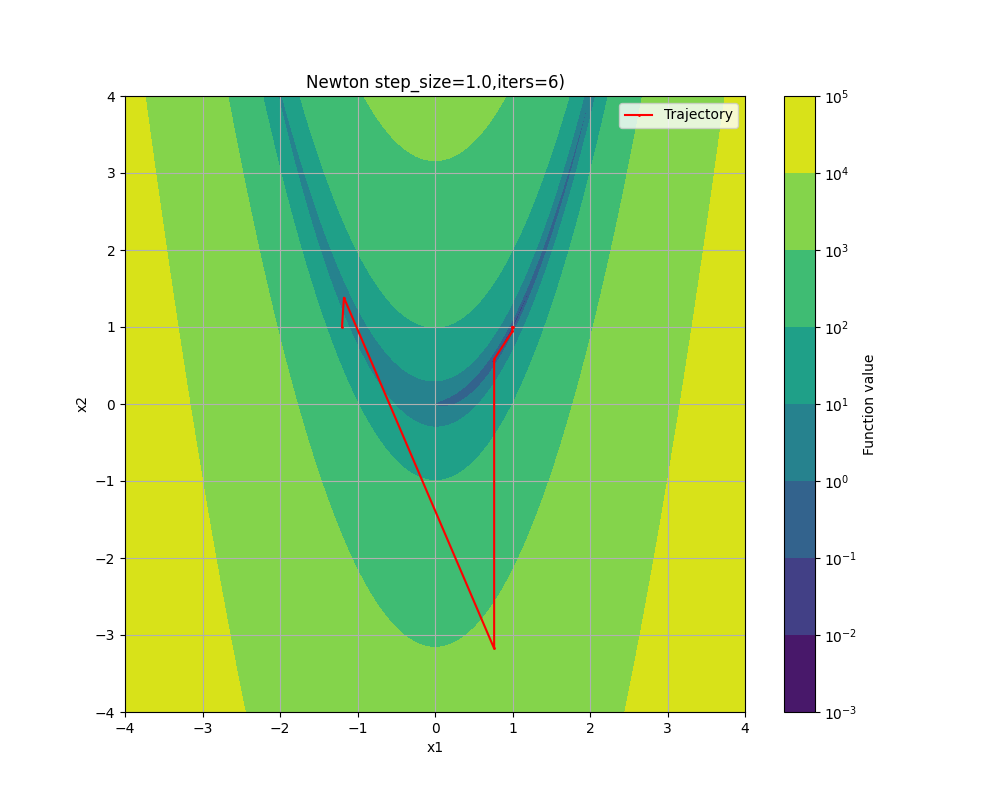
\includegraphics[width=.9\textwidth]{newton.png}
  \caption{Newton's method with fixed step size converges in 6 iterations}
  \label{fig:newton_fixed}
\end{figure}

\subsection*{Armijo Newton}
Now, we switch to using the Armijo step size rule for Newton's method. The
Armijo step size is computed by checking increasing integer values of $s$ until
the Armijo condition is satisfied.
\begin{minted}[fontsize=\small]{python}
def compute_armijo_s(x, a, b):
    """Compute the Armijo step size."""
    s = 1

    f, grad, hessian = rosenbrock(x)
    p = np.linalg.solve(hessian, grad)
    f_next = rosenbrock(x - b**s * p)[0]

    while f_next - f >= - a * b**s * np.dot(grad, p):
        s += 1
        f_next = rosenbrock(x - b**s * p)[0]

    return s


def newton_armijo(x0, a, b, tolerance, max_iter=1e6):
    """Newton's method with a fixed step size."""
    x = x0
    trajectory = [x.copy()]

    iter = 0
    # Compute the initial function value and gradient
    _, grad, hessian = rosenbrock(x)
    while np.linalg.norm(grad) > tolerance and iter < max_iter:
        # Check the armijo condition
        s = compute_armijo_s(x, a, b)

        # Move in the direction of the negative gradient
        x -= b**s * np.linalg.solve(hessian, grad)
        # Update the trajectory
        trajectory.append(x.copy())

        # Compute the next values and iterate
        _, grad, hessian = rosenbrock(x)
        iter += 1
    return np.array(trajectory)
\end{minted}

Running the code for the Rosenbrock function as before, the output is plotted in
\ref{fig:newton_armijo}, where we now see that the trajectory is staying within
the minimizing region of the function. The method converges in $74$ iterations,
so there is a tradeoff here between the number of iterations and the
conditioning of the descent method.

\begin{figure}[H]
  \centering
  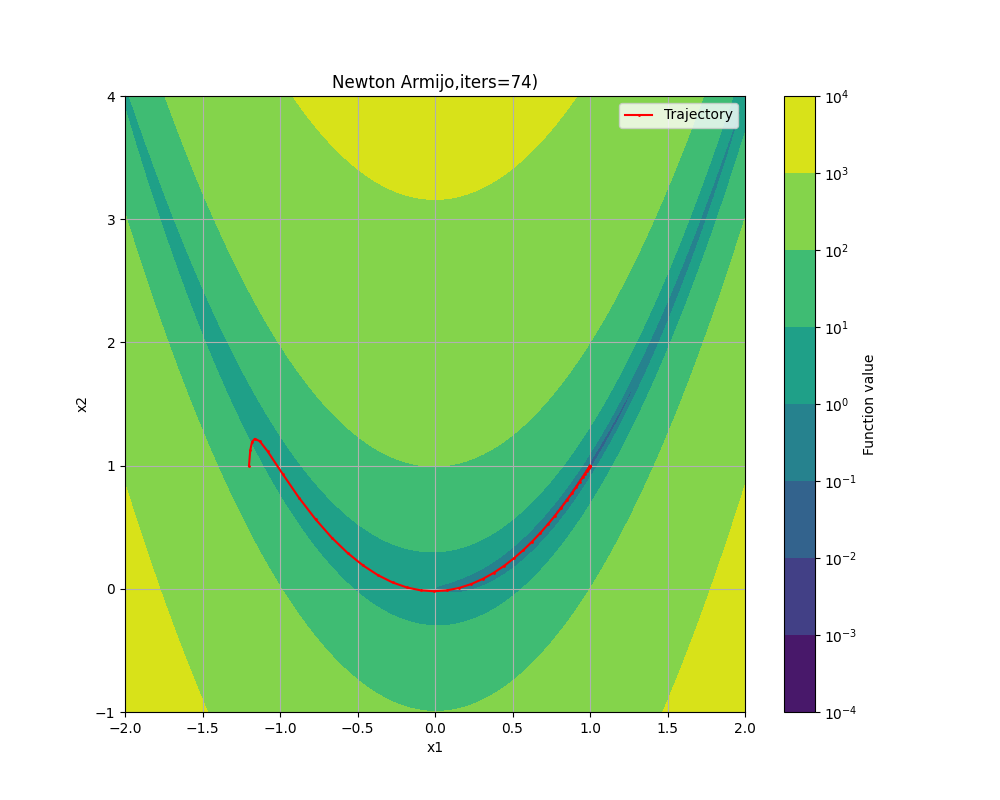
\includegraphics[width=.9\textwidth]{newton_armijo.png}
  \caption{Newton's method with Armijo converges in 74 iterations}
  \label{fig:newton_armijo}
\end{figure}

\subsection*{Armijo Gradient Descent}
Finally, we have the case of gradient descent with Armijo step size. The code
for this is a simplified verson of the Newton's method with Armijo step size, as
we only need to use the gradient of the function and not the Hessian.

\begin{minted}[fontsize=\small]{python}
def compute_armijo_s(x, a, b):
    """Compute the Armijo step size."""
    s = 1

    f, grad, _ = rosenbrock(x)
    f_next = rosenbrock(x - b**s * grad)[0]

    while f_next - f >= - a * b**s * np.dot(grad, grad):
        s += 1
        f_next = rosenbrock(x - b**s * grad)[0]

    return s


def gradient_descent_armijo(x0, a, b, tolerance, max_iter=100000):
    """Perform gradient descent with a fixed step size."""
    x = x0
    trajectory = [x.copy()]

    iter = 0
    # Compute the initial function value and gradient
    _, grad, _ = rosenbrock(x)
    while np.linalg.norm(grad) > tolerance and iter < max_iter:
        # Check the armijo condition
        s = compute_armijo_s(x, a, b)

        # Move in the direction of the negative gradient
        x -= b**s * grad
        # Update the trajectory
        trajectory.append(x.copy())

        # Compute the next values and iterate
        _, grad, _ = rosenbrock(x)
        iter += 1
    return np.array(trajectory)
\end{minted}

Running the code for the Rosenbrock function as before, the output is plotted in
\ref{fig:grad_armijo}, where we see that the trajectory enters the minimizing
region, but makes a large jump towards the absolute minimum of teh function. It
then converges very slowly to the minimum over the remaining distances, taking
$1131$ iterations to converge. This makes sense as the gradient method is not
accounting for the low curvature of the function when inside the minimizing
basin, and so it is taking very small steps to converge to the minimum.

\begin{figure}[H]
  \centering
  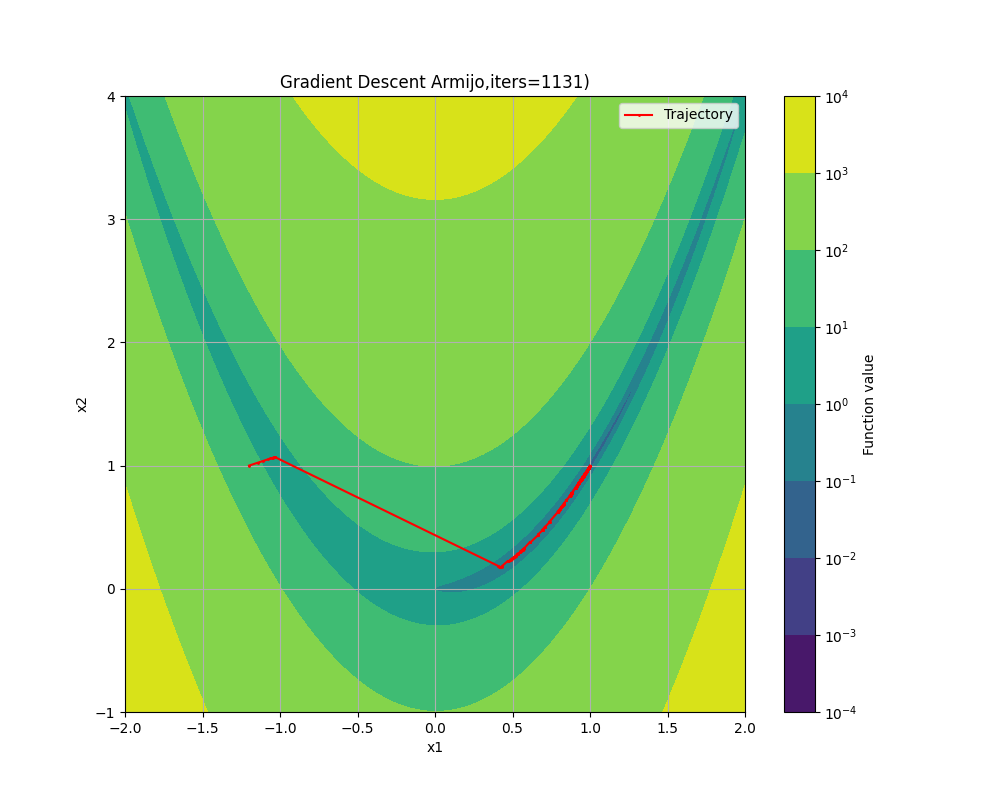
\includegraphics[width=.9\textwidth]{grad_armijo.png}
  \caption{Gradient descent with Armijo converges in 1131 iterations}
  \label{fig:grad_armijo}
\end{figure}


\end{document}

